\documentclass[titlepage]{article}
\usepackage[ukrainian]{babel}
\usepackage{listings}
\usepackage{amsmath}
\usepackage{fontspec}
\setmainfont{Times New Roman}
\usepackage{setspace}
%\spacing{1.7}
\usepackage{fancyhdr}
\usepackage{titling}
\usepackage[a4paper, top = 20mm, bottom = 20mm, left = 25mm, right = 15mm]{geometry}
\usepackage{graphics}

\lstset{
	basicstyle=\large,
	breaklines = true,
	language = matlab,
	breakatwhitespace = true,
	numbers = left,
	numberstyle = \tiny,
	columns = flexible,
	frame=tb,
	tabsize=4
}

\makeatletter
\renewcommand\normalsize{%
\@setfontsize\normalsize{14pt}{15pt}}
\makeatother

\newcommand\makelisting[1]{\lstinputlisting[title=#1]{../#1} \vspace{1cm}}

\preauthor{\begin{flushright}}
\postauthor{\end{flushright}}

\fancypagestyle{empty}{%
	\renewcommand{\headrulewidth}{0pt}
	\cfoot{\normalsize2016}
	\chead{\uppercase{київський національний університет імені тараса шевченка}}
}

\begin{document}
\title{\LARGE Робота учбової практики}
\author{\vspace{12cm}Виконав: \protect\\ студент 4-го курсу \protect\\ спеціальність математика \protect\\ Колінько Микола Миколайович}
\date{}
\maketitle

\section{Постановка задачі}

Необхідно побудувати інтерполяційний сплайн $S(x, u)$ другого степеня дефекту 1, з крайовими умовами типу 4.
\section{Теоретичні відомості}

Для побудови системи рівнянь для коефіціентів використаємо другі похідні $2a_i = M_i = S^{''}(X_i, u)$. Використовуючи рівність поділених різниць сплайну та інтерпольованої функціі в точках $X$ отримуємо обмеження на $M_i$:

\begin{equation}
\begin{split}
&h_{i-1}M_{i-1} + 3(h_{i-1} + h_i)M_i + h_iM_i = 8u(X_{i-1};X_i;X_{i+1})(h_{i-1} + h_i);\\
&h_{i-1}M_{i-1} + 3(h_{i-1} + h_i)M_i + h_iM_i = 8(u(X_i; X_{i+1}) - u(X_{i-1}; X_i)).
\end{split}
\nonumber
\end{equation}

Де $h_i = X_{i+1} - X_i$. Тоді (враховуючи 4 Тип обмежень) отримуємо систему рівнянь:

\begin{equation}
\begin{split}
&-M_1 + M_2= 0;\\
&h_{i-1}M_{i-1} + 3(h_{i-1} + h_i)M_i + h_iM_i = 8(u(X_i; X_{i+1}) - u(X_{i-1}; X_i)), i = \overline{2,n-1};\\
&M_{n-1} - M_{n} = 0.
\end{split}
\nonumber
\end{equation}

Для якої можна записати матрицю
\[\left(\begin{array}{ccccc|c}
-1 & 1 & 0 & \ldots & 0 & 0\\
h_1 & 3(h_1 + h_2) & h_2 & \ldots& 0  & 8(u(X_2; X_3) - u(X_1; X_2))\\
\ldots &\ldots &\ldots &\ldots &\ldots & \ldots\\
\ldots & 0 &h_{n-2} & 3(h_{n-2} + h_{n- 1}) & h_{n-1} & 8(u(X_{n-1}; X_n) - u(X_{n-2}; X_{n-1})\\
0 & \ldots & 0  & -1 & 1 & 0
\end{array}\right)\]
Систему рівнянь розв'язуємо методом лівої прогонки.

Для обрахування саме коефіціентів сплайну використовуються наступні формули:
\begin{equation}
\begin{split}
&a_i = \frac{M_i}{2};\\
&c_i = u_i;\\
&b_1 = u(X_1, X_2) - \frac{1}{8}h_1(3M_1 + M_2);\\
&b_i = u(X_{i-1};X_i) + \frac{1}{8}h_1(M_{i-1} + 3M_i), i=\overline{2,n}.
\end{split}
\nonumber
\end{equation}
\vspace{20cm}
\section{Код}

Функція, що здійснює перевірку правильності побудови сплайну: побудову графіків та розрахунок сіткової норми.
\makelisting{main.m}
\vspace{20cm}
Функція, що здійснює побудову сплайна.
\makelisting{CreateSpline.m}
\vspace{20cm}
Побудова матриці відповідно до методу побудови системи лінійний рівнянь, що зазначений в умові.
\makelisting{CreateMatrix.m}
Розв'язання системи лінійних рівнянь за визначеним в умові методом
\makelisting{Solve.m}
Формування коефіцієнтів сплайну.
\makelisting{FormSpline.m}
Нижче наведений результат роботи програми:
\begin{figure}[h]
\hspace{-3cm}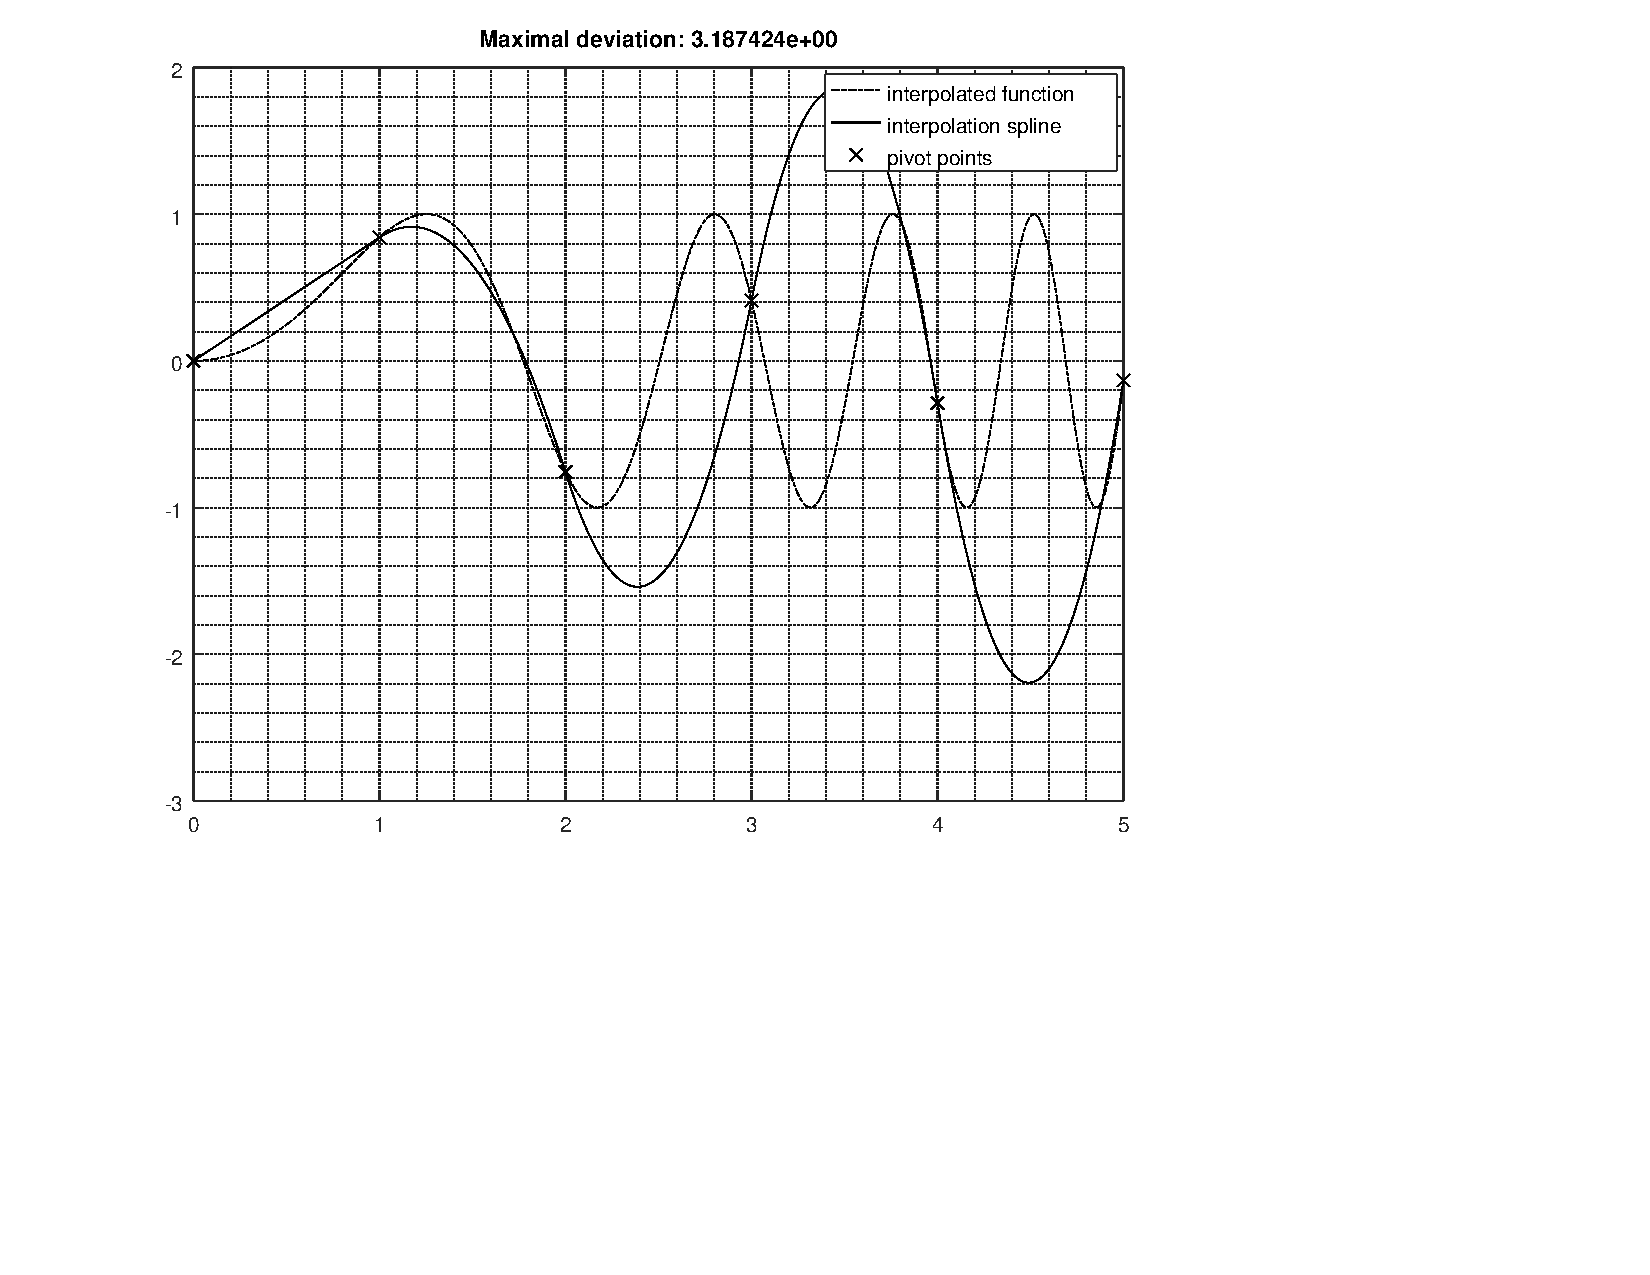
\includegraphics[page=1]{../result.pdf}
\end{figure}
\begin{figure}[h]
\hspace{-3cm}\includegraphics[page=2]{../result.pdf}
\end{figure}
\end{document}
